\section{Protocol Specification}

The protocol portion of Taxicoin is designed to be open. As such, anybody should be able to implement it in their own software. The following section of this document should be sufficient to do so.

\subsection{Methods}

Each of these methods is intended to be part of a smart contract. When one is called, it will modify the state of the contract, and/or return a value.

The specified arguments are to be supplied when calling that function of the contract, with the types representing built-in Solidity language types. The \textit{payable} keyword indicates that a method accepts a transaction with a currency value attached. In instances where the preconditions for a method are not met, the method will revert and the state will be unmodified.

\subsubsection{Driver Advertise}

\begin{description}[leftmargin=8em,style=nextline]
	\item [Description]
		Takes a deposit from a driver and publishes their location and public key.
	\item [Arguments]
		Latitude: String \\
		Longitude: String \\
		Public Key: String
	\item [Payable]
		Driver deposit
	\item [Preconditions]
		User must not be currently on a journey, either as a driver or rider. Deposit must either have been already provided, or sent with this transaction.
	\item [Postconditions]
		The driver's location and public key are published, and the value of the deposit provided by the driver is recorded. If any deposit over the required amount was provided with the transaction, the excess is returned.
\end{description}

\subsubsection{Driver Advert Revoke}

\begin{description}[leftmargin=8em,style=nextline]
	\item [Description]
		Removes an active driver's advertisement.
	\item [Arguments]
		None
	\item [Payable]
		No
	\item [Preconditions]
		User must be advertised as a driver.
	\item [Postconditions]
		The driver is removed from the list of active drivers, indicating that riders should not send job proposals to this driver. The previously supplied deposit is not returned.
\end{description}

\subsubsection{Rider Create Journey}

\begin{description}[leftmargin=8em,style=nextline]
	\item [Description]
		Accepts a quoted fare for a journey as a rider and forms the rider's part of a contract between driver and rider. Intended to be called after an off-chain negotiation with \lstinline{job} and \lstinline{quot} messages.
	\item [Arguments]
		Driver Address: address \\
		Fare: uint, value in \textit{wei} $n > 0$ \\
		Public Key: String
	\item [Payable]
		Fare plus rider deposit
	\item [Preconditions]
		The user at the provided address must be an actively advertised driver, and not currently on a journey. The user calling this method must not be an actively advertised driver, nor be part of a journey as either rider or driver. The full rider deposit, plus an amount equal to the provided \lstinline{fare} must have been provided with this transaction.
	\item [Postconditions]
		The rider's intent to travel with the specified driver at the specified price is published. At this stage, the agreement is not binding until the driver accepts, before which the journey may be cancelled, with the rider deposit and fare being returned in full.
\end{description}

\subsubsection{Rider Cancel Journey}

\begin{description}[leftmargin=8em,style=nextline]
	\item [Description]
		Cancels a journey which has not yet been accepted by a driver.
	\item [Arguments]
		None
	\item [Payable]
		No
	\item [Preconditions]
		Rider must be part of a journey, for which the driver has not already accepted.
	\item [Postconditions]
		The rider is removed from the journey. From this point it is no longer possible for the driver to accept the journey. The rider's deposit and fare are returned.
\end{description}

\subsubsection{Driver Accept Journey}

\begin{description}[leftmargin=8em,style=nextline]
	\item [Description]
		Formally accepts a job as a driver, committing both the rider and driver to its completion.
	\item [Arguments]
		Rider Address: address \\
		Fare: uint, value in \textit{wei} $n > 0$
	\item [Payable] 
		No
	\item [Preconditions]
		Driver must be actively advertised and have provided the driver deposit. Rider must have formally created a journey with the driver set to the caller of this method, and the fare of equal value to the argument provided.
	\item [Postconditions]
		The driver is marked as being on a journey with the specified rider. From this point, the journey is considered to be in progress, and any attempt to change any aspect of the journey will require an agreement to be made between both rider and driver.
\end{description}

\subsubsection{Complete Journey}

\begin{description}[leftmargin=8em,style=nextline]
	\item [Description]
		Marks the current journey as completed, as either the rider or driver.
	\item [Arguments]
		Rating: uint8, $1 \leq n \leq 255$ with 255 being the \enquote{best}
	\item [Payable] No
	\item [Preconditions]
		The caller of the method must either be a driver or rider who is currently on a journey.
	\item [Postconditions]
		The caller of the method is marked as having completed the journey, however they are still part of this journey until the other user has also called this method. The rating for the other user is stored. If the other party has already called this method, then the ratings for both parties are applied to their overall rating, and the journey is formally completed. The rider and driver deposits are returned, and the fare transferred to the driver. However, in cases where the fare is zero (only possible where the fare has been altered during a journey to indicate that the journey should be cancelled), the driver's deposit is not returned.
\end{description}

\subsubsection{Driver Propose Fare Alteration}

\begin{description}[leftmargin=8em,style=nextline]
	\item [Description]
		Formally proposes the alteration of the fare for a journey. Intended to be called after an off-chain negotiation with \lstinline{Propose Fare Alteration} messages.
	\item [Arguments]
		New Fare: uint, value in \textit{wei}
	\item [Payable]
		No
	\item [Preconditions]
		The user calling the method must be a driver, and currently be on a journey.
	\item [Postconditions]
		The driver's proposed new fare is recorded. The new fare does not take effect until the rider calls the \lstinline{Confirm Fare Alteration} method.
\end{description}

\subsubsection{Rider Confirm Fare Alteration}

\begin{description}[leftmargin=8em,style=nextline]
	\item [Description]
		Confirms the alteration of the fare for a journey.
	\item [Arguments]
		New Fare: uint, value in \textit{wei}
	\item [Payable]
		Difference between old and new fares, if new is higher
	\item [Preconditions]
		The user calling the method must be currently on a journey. Driver must have previously agreed the same new fare with the \lstinline{Alter Fare} method. In the case that the new fare is higher, the difference must have been provided with this transaction.
	\item [Postconditions]
		The new value for the fare for the journey is recorded. In the case that the new fare is lower, the difference is returned to the rider. If the new fare is zero, the journey is considered to be cancelled - the journey may now be completed with the rider's deposit being returned, and no fare being paid to the driver.
\end{description}

\subsubsection{Get User Type}

\begin{description}[leftmargin=8em,style=nextline]
	\item [Description]
		Returns an integer representing the type of user at the provided address.
	\item [Arguments]
		User Type: uint8
	\item [Payable]
		No
	\item [Preconditions]
		None
	\item [Postconditions]
		Returns an integer between 0 and 3, representing the enum \{ None, Driver, ActiveDriver, Rider \}.
\end{description}

\subsubsection{Get Driver}

\begin{description}[leftmargin=8em,style=nextline]
	\item [Description]
		Returns the details of the driver at the given address.
	\item [Arguments]
		Driver Address: address
	\item [Payable]
		No
	\item [Preconditions]
		None
	\item [Postconditions]
		If the address provided is of a user who has previously (or is currently) advertised as a driver, the details of the driver will be returned.
		
		Otherwise, all zero-values will be returned.
\end{description}

\subsubsection{Get Next Driver}

\begin{description}[leftmargin=8em,style=nextline]
	\item [Description]
		Returns the details of the driver next in the list of advertised drivers after the given address.
	\item [Arguments]
		Driver Address: address
	\item [Payable]
		No
	\item [Preconditions]
		None
	\item [Postconditions]
		If the address provided is of a user who has previously (or is currently) advertised as a driver, the details of the next driver in the list will be returned.
		
		If the zero-address (\lstinline{0x0}) is provided, the first driver in the list is returned.
		
		If the address provided is for the last driver in the list, the zero-address is returned.
\end{description}

\subsubsection{Get Previous Driver}

\begin{description}[leftmargin=8em,style=nextline]
	\item [Description]
		Returns the details of the driver previous in the list of advertised drivers after the given address.
	\item [Arguments]
		Driver Address: address
	\item [Payable]
		No
	\item [Preconditions]
		None
	\item [Postconditions]
		If the address provided is of a user who has previously (or is currently) advertised as a driver, the details of the previous driver in the list will be returned.
		
		If the zero-address (\lstinline{0x0}) is provided, the last driver in the list is returned.
		
		If the address provided is for the first driver in the list, the zero-address is returned.
\end{description}

\subsubsection{Get Rider}

\begin{description}[leftmargin=8em,style=nextline]
	\item [Description]
		Returns the details of the rider at the given address.
	\item [Arguments]
		Rider Address: address
	\item [Payable]
		No
	\item [Preconditions]
		None
	\item [Postconditions]
		If the address provided is of a user who has previously used (or is currently using) the system as a rider, the details of the rider will be returned.
		
		Otherwise, all zero-values will be returned.
\end{description}

\subsection{Messages}

Driver and rider user clients should be listening for the following messages, where applicable. These messages are communicated via the Whisper protocol.

Message topics are always a length of 4 bytes (4 ASCII characters), therefore any topics listed here of a length less than 4 byes are right-padded with spaces.

\subsubsection{Job Proposal}

\begin{description}[leftmargin=6em,style=nextline]
	\item [Topic]
		\lstinline{job}
	\item [Purpose]
		This message is sent by a rider to a prospective driver, indicating that they wish to make the described journey. It is intended to be sent to advertised drivers matching a specified criteria, e.g. within a certain distance, with at least a certain reputation.
		
		However the sending of these messages is not intended to be carried out manually by the user -- rather there is an automated process which fetches the list of active drivers and determines which to propose to.
	\item [Response]
		Should a driver be interested in a proposal, they respond with a quote message.
	\item [Payload]
		Please see below.
\end{description}

\lstinputlisting{res/job-message.json}

\subsubsection{Driver Quote}

\begin{description}[leftmargin=6em,style=nextline]
	\item [Topic]
		\lstinline{quot}
	\item [Purpose]
		This message is sent by a driver as a response to a job proposal. It contains the network address of the driver, as well as the fare for which the driver is willing to take on the job. At this point, the quote is not binding.
		
		Quote messages with a fare of -1 are considered to be a rejection, indicating that the driver does not wish to accept this job.
	\item [Response]
		If the rider chooses to accept the quote, they next call the create journey method, and respond with a \lstinline{Journey Created} message.
	\item [Payload]
		Please see below.
\end{description}

\lstinputlisting{res/quote-message.json}

\subsubsection{Journey Created}

\begin{description}[leftmargin=6em,style=nextline]
	\item [Topic]
		\lstinline{crea}
	\item [Purpose]
		This message is sent by a rider to a driver after they have created a journey. This is an indication that the rider has accepted the driver's quote.
	\item [Response]
		The driver should next call the \lstinline{Driver Accept Journey} method, and respond with a \lstinline{Journey Accepted} message.
	\item [Payload]
		Please see below.
\end{description}

\lstinputlisting{res/created-message.json}

\subsubsection{Journey Accepted}

\begin{description}[leftmargin=6em,style=nextline]
	\item [Topic]
		\lstinline{accp}
	\item [Purpose]
		This message is sent by a driver to a rider, after they have formally accepted the rider's journey, to indicate that both parties are now on a journey.
	\item [Response]
		None
	\item [Payload]
		Please see below.
\end{description}

\lstinputlisting{res/accepted-message.json}

\subsubsection{Driver Location}

\begin{description}[leftmargin=6em,style=nextline]
	\item [Topic]
		\lstinline{lctn}
	\item [Purpose]
		Sends the location of the driver to the rider with whom they are currently on a journey with. Allows the rider's client to display how far the driver is from the pickup location.
	\item [Response]
		None
	\item [Payload]
		Please see below.
\end{description}

\lstinputlisting{res/location-message.json}

\subsubsection{Journey Completed}

\begin{description}[leftmargin=6em,style=nextline]
	\item [Topic]
		\lstinline{cmpl}
	\item [Purpose]
		This message is sent to the other party when either one calls the \lstinline{Complete Journey} method. It indicates that the other should also (or dispute it). If the other party has already completed the journey, then this message indicates that the journey is fully complete.
	\item [Response]
		None
	\item [Payload]
		None
\end{description}

\subsubsection{Propose Fare Alteration}

\begin{description}[leftmargin=6em,style=nextline]
	\item [Topic]
		\lstinline{nfar}
	\item [Purpose]
		This message is sent to the other party to indicate that the user wishes to alter the fare for the current journey.
	\item [Response]
		If the message is received by a driver for the first time, unprompted, they may either agree with the new proposed fare, and formally propose the new fare with the \lstinline{Propose Fare Alteration} method, or reject the new fare by sending a message of this type with an alternate fare.
		
		If the message is received by a driver for the second time, after agreeing to the proposed new fare, and the value in this message is unchanged, this indicates that the rider has called the \lstinline{Rider Confirm Fare Alteration} method, and the new fare has been applied. No further response is sent. However if the fare was changed, the driver may act as if this is the first such message (see above).
		
		If the message is received by a rider for the first time, unprompted, the rider may either agree to the new fare, and respond with a message of the same type with an unchanged value, or they may disagree and respond with their proposed new fare.
		
		If the message is received by a rider for the second time, after agreeing to the proposed new fare, and the value is unchanged, this indicates that the driver has called the \lstinline{Propose Fare Alteration} method, and that the rider should call the \lstinline{Rider Confirm Fare Alteration} method. They then respond with a message of this type, with the fare value unchanged.
	\item [Payload]
		Please see below.
\end{description}

\lstinputlisting{res/new-fare-message.json}

\subsection{Contract Solidity Interface}

The above methods can be translated to a Solidity interface, which should be conformed to for all Ethereum-based contracts implementing the Taxicoin protocol. This aids the goal of creating an open ecosystem as, in theory, if all implementations conform to this standard, any client should be able to work with any contract implementation.

\lstinputlisting[language=Solidity]{../contracts/ITaxicoin.sol}

\pagebreak
\subsection{Process Flow Diagram}

This describes the possible routes of interaction through the system.

\begin{figure*}[h!]
% include shapes and arrows for flow charts and set up
\usetikzlibrary{shapes.geometric, arrows}
\tikzstyle{startstop} = [rectangle, rounded corners, minimum width=3cm, text width=3cm, minimum height=1cm,text centered, draw=black, fill=red!30]
\tikzstyle{io} = [trapezium, trapezium left angle=70, trapezium right angle=110, minimum width=3cm, text width=3cm, minimum height=1cm, text centered, draw=black, fill=blue!30]
\tikzstyle{process} = [rectangle, minimum width=3cm, text width=3cm, minimum height=1cm, text centered, draw=black, fill=orange!30]
\tikzstyle{decision} = [diamond, aspect=1.2, minimum width=3cm, text width=2cm, minimum height=1cm, text centered, draw=black, fill=green!30]
\tikzstyle{arrow} = [thick,->,>=stealth]

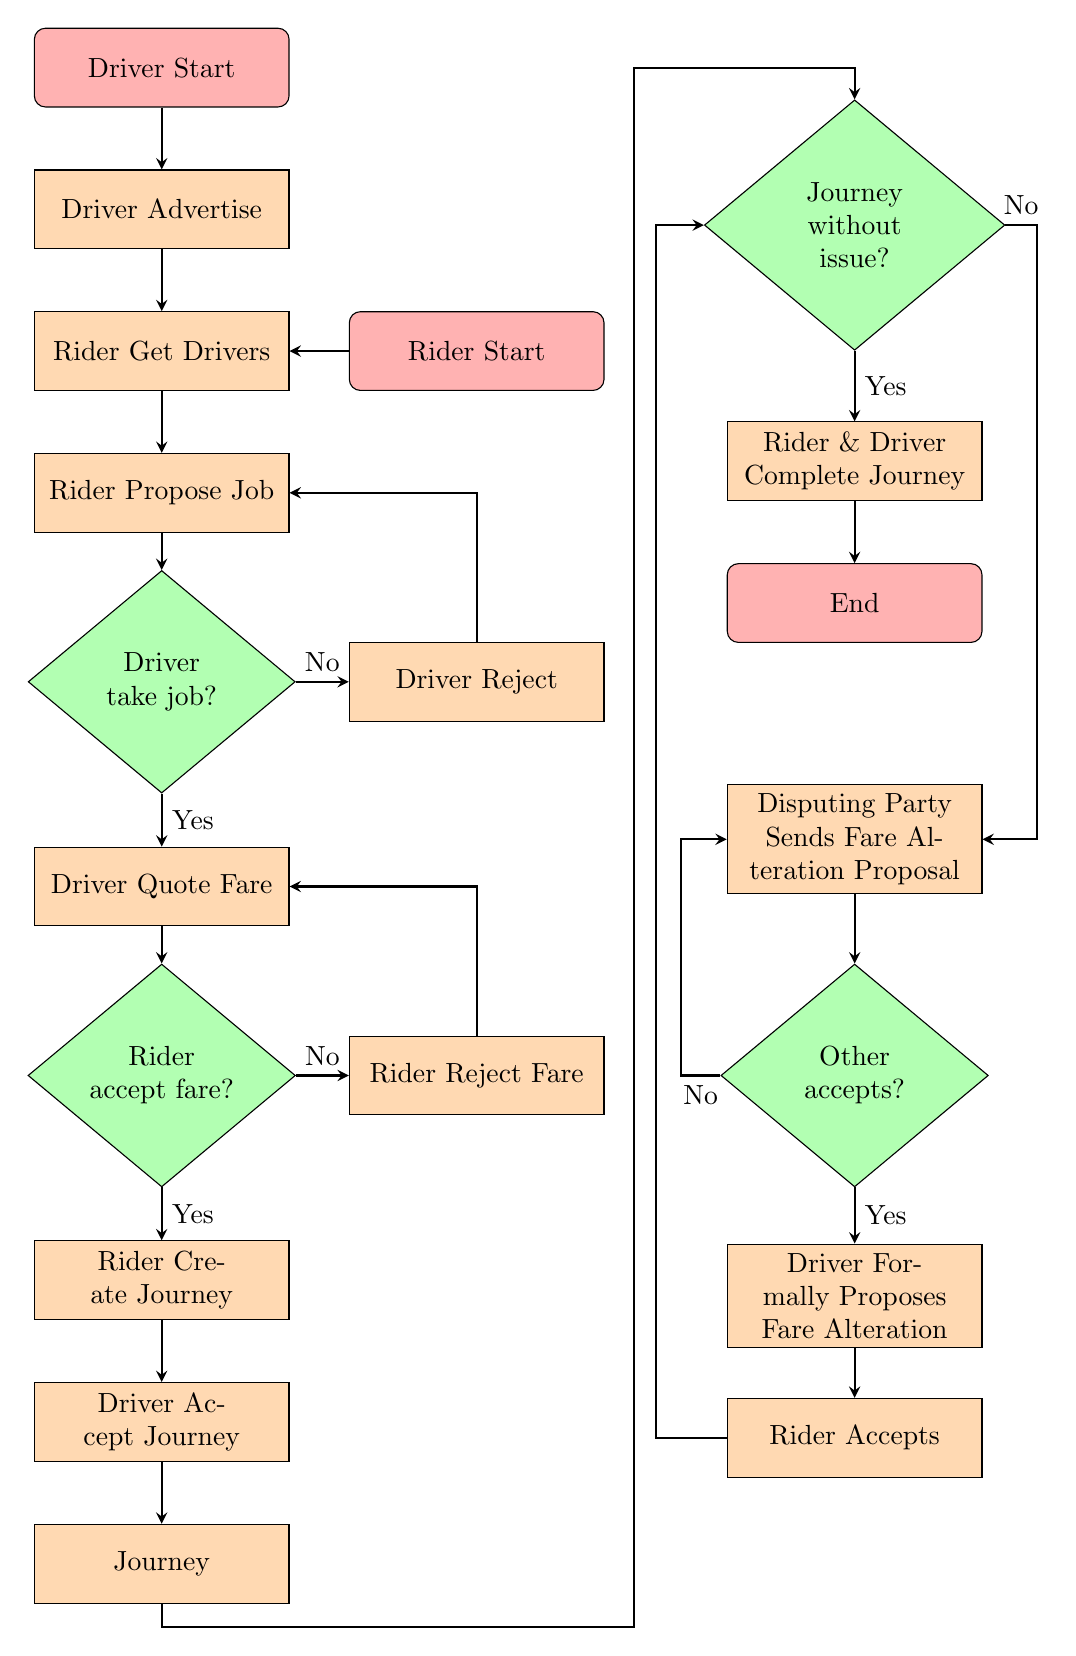
\begin{tikzpicture}[node distance=1.8cm]
	\node (n0) [startstop] {Driver Start};
	\node (n1) [process, below of=n0] {Driver Advertise};
	\node (n2) [process, below of=n1] {Rider Get Drivers};
	\node (n3) [startstop, right of=n2, xshift=2.2cm] {Rider Start};
	\node (n4) [process, below of=n2] {Rider Propose Job};
	\node (n5) [decision, below of=n4, yshift=-0.6cm] {Driver take job?};
	\node (n6) [process, right of=n5, xshift=2.2cm] {Driver Reject};
	\node (n7) [process, below of=n5, yshift=-0.8cm] {Driver Quote Fare};
	\node (n8) [decision, below of=n7, yshift=-0.6cm] {Rider accept fare?};
	\node (n9) [process, right of=n8, xshift=2.2cm] {Rider Reject Fare};
	\node (n10) [process, below of=n8, yshift=-0.8cm] {Rider Create Journey};
	\node (n11) [process, below of=n10] {Driver Accept Journey};
	\node (n12) [process, below of=n11] {Journey};
	\node (n13) [decision, right of=n0, xshift=7cm, yshift=-2cm] {Journey without issue?};
	\node (n14) [process, below of=n13, yshift=-1.2cm] {Rider \& Driver Complete Journey};
	\node (n15) [startstop, below of=n14] {End};
	\node (n16) [process, below of=n15, yshift=-1.2cm] {Disputing Party Sends Fare Alteration Proposal};
	\node (n17) [decision, below of=n16, yshift=-1.2cm] {Other accepts?};
	\node (n18) [process, below of=n17, yshift=-1cm] {Driver Formally Proposes Fare Alteration};
	\node (n19) [process, below of=n18] {Rider Accepts};
	
	\draw [arrow] (n0) -- (n1);
	\draw [arrow] (n1) -- (n2);
	\draw [arrow] (n3) -- (n2);
	\draw [arrow] (n2) -- (n4);
	\draw [arrow] (n4) -- (n5);
	\draw [arrow] (n5) -- node[anchor=south] {No} (n6);
	\draw [arrow] (n6) |- (n4);
	\draw [arrow] (n5) -- node[anchor=west] {Yes} (n7);
	\draw [arrow] (n7) -- (n8);
	\draw [arrow] (n8) -- node[anchor=south] {No} (n9);
	\draw [arrow] (n9) |- (n7);
	\draw [arrow] (n8) -- node[anchor=west] {Yes} (n10);
	\draw [arrow] (n10) -- (n11);
	\draw [arrow] (n11) -- (n12);
	
	\draw [arrow] (n12.south) |- ++(6cm,-3mm) -- ++(0,19.8cm) -| (n13.north);
	
	\draw [arrow] (n13) -- node[anchor=west] {Yes} (n14);
	\draw [arrow] (n14) -- (n15);
	
	\draw [arrow] (n13.east) -- node[anchor=south] {No} ++(4mm,0) |- (n16.east);
	\draw [arrow] (n16) -- (n17);
	\draw [arrow] (n17) -- node[anchor=west] {Yes} (n18);
	\draw [arrow] (n17.west) -- node[anchor=north] {No} ++(-5mm,0) |- (n16.west);
	\draw [arrow] (n18) -- (n19);
	\draw [arrow] (n19.west) -- ++(-9mm,0) |- (n13.west);
\end{tikzpicture}
\end{figure*}
